\section{Sensitivity Forecast}\label{sec:sens}
%%%%%%%%%%%%%%%


\subsection{Astrophysical sources}

As a first step, we determine whether the anisotropy and the cross-correlation signals from unresolved astrophysical sources are detectable. As a statistical figure of merit, we adopt the signal-to-noise ratio (SNR), defined, for the cross-correlation, as
\begin{equation}
    \textrm{SNR} = \sqrt{\sum_{\ell, i} \left(\frac{C_{\ell, i}^{\gamma g}}{\varDelta C_{\ell, i}^{\gamma g}}\right)^2}\;,
    \label{eq:SNR2}
\end{equation}
%
where the sum runs over all the multipoles $\ell$ considered in the analysis and all energy bins $i$. For the auto-correlation, the formula is analogous but using $C_{\ell, i}^{{\gamma \gamma}}$ and $\varDelta C_{\ell,i}^{\gamma \gamma}$.

To be more specific, the energy bins adopted in our analysis are 16, logarithmically spaced in the 30 GeV – 30 TeV range.
The sum over multipoles extends from $\ell = 10$ up to $\ell = 1000$. The lower value $\ell = 10$ is adopted to avoid the largest angular scales (i.e., lowest multipoles),
where the $\gamma$-ray Galactic foreground is the dominant emission, and, if not properly modeled and removed, can create some artifact in the reconstructed signal, especially in the auto-correlation. This issue is, however, mostly of concern for a real data analysis like the one in \cite{Fermi-LAT:2018udj}, where we refer the reader for further details. In our forecast, starting the sum from $\ell=10$ or $\ell=1$ has a negligible impact on the final results.
At the same time, we do not consider very large multipoles, since the (energy-dependent) angular resolution of the $\gamma$-ray detector prevents us from accessing information on angular scales which are much smaller than its point-spread-function (PSF). The CTAO PSF has been determined through a Monte Carlo simulation of the detector and is shown in Fig. \ref{fig:PSF_Beam} in Appendix \ref{app:model}, together with its harmonic space transform $B_\ell$, which enters in the expression for the variance $\varDelta C_{\ell, i}^{\gamma g}$ of Eq. (\ref{eq:Delta}). From Fig. \ref{fig:PSF_Beam} we can see that for multipoles above about 1000 the beam function $B_\ell$ sharply decreases, thus inflating the variance and making those large multipoles irrelevant for the SNR.

The results for 3 hours and 50 hours of observation time are shown in \cref{table:SNR}, for both LISP and HSP source classes, and for both the auto-correlation and cross-correlation APS with the 2MASS galaxy catalog. We find that a purely astrophysical signal from unresolved sources can reach at most (for 50 hours of observation) only a marginal evidence of $\textrm{SNR} \simeq 0.9$ in the autocorrelation, and about $0.16$ in the cross-correlation case.   
These values of SNR correspond to the HSP blazars, whose hard spectra are better suited to the CTAO energy range. The SNR is even smaller for LISPs, whose softer spectra result in a poorer overlap with the CTAO sensitivity. 

As an aside comment, let us note that this is not necessarily a negative result: it simply reflects the fact that the expected sensitivity of CTAO to point-source detection would be good enough to resolve a large fraction of blazars, thereby reducing the auto- and cross-correlation APS of the \textsl{unresolved} population. In this case, it would be actually convenient and sufficient to perform auto- and cross-correlation APS analyses directly on the catalog of resolved sources in order to study their anisotropy properties. 

\begin{table}[t!]
\centering
\begin{tabular}{m{0.15\textwidth}  m{0.15\textwidth}  m{0.15\textwidth}} 
 \hline
 SNR for $3\,\textrm{hrs}$ & Auto-correlation & Cross with 2MASS \\ [0.5ex]
 \hline
 LISP &  0.042 &   $8.2\cdot 10^{-3}$ \\ [0.5ex]
 HSP &  0.31 &  0.1 \\  [1.5ex]
 \hline \hline
  SNR for $50\,\textrm{hrs}$ & Auto-correlation & Cross with 2MASS \\ [0.5ex]
 \hline
 LISP &  0.18 &  0.022 \\ [0.5ex]
 HSP &  0.9 &  0.16\\ [1ex]
 \hline
\end{tabular}
\caption{The predicted signal-to-noise ratios for 3-hours and 50-hours observations of LISP and HSP source classes, obtained for both $\gamma$-rays auto-correlation and cross-correlation with the 2MASS galaxy catalog. 
}
\label{table:SNR}
\end{table}

\begin{table}[t!]
\centering
\begin{tabular}{m{0.15\textwidth} m{0.15\textwidth} m{0.15\textwidth}} 
\hline
 SNR $50\,\textrm{hrs}$ low res & Auto-correlation & Cross with 2MASS 
 \\ [0.5ex]
 \hline
 LISP &  0.7 &   0.033 \\ [0.5ex]
 HSP &  5.1 &  0.41 \\  [1ex]
 \hline
\end{tabular}
\caption{Same as \cref{table:SNR} but for $50\,\textrm{hrs}$-observations, assuming a source detection threshold approximately three times worse than in \cref{table:SNR}. This illustrates the strong dependence of the auto-correlation signal on the point source detection threshold.}
\label{table:SNR-mix}
\end{table}

However, we wish to stress that this result, i.e., the fact that CTAO sensitivity would be enough to resolve a significant fraction of blazars, 
strongly depends on the assumed point-source sensitivity of the detector, which for CTAO {remains subject to considerable uncertainty}  (as discussed in \cref{sec:CTA}). This is because the {final configuration and specifications of CTAO have not yet been fully settled.}  For example, the point-source sensitivity {differs significantly between}  CTAO-North and CTAO-South \cite{CTAConsortium:2018tzg}, and at the moment the relative share of North and South array observations to the survey is still undecided. To assess the capabilities of CTAO for the study of anisotropies of point-sources even in the case that the point-source sensitivity is worse than the nominal case derived and adopted in this paper, we repeat the analysis for point-sources by assuming a degraded point-source detection capability. Table \ref{table:SNR-mix} shows the SNR obtained for 50 hrs of observations, assuming a source detection threshold approximately three times worse than in the nominal case of Table \ref{table:SNR}. This has been achieved by using the 50 hrs exposure with a point-source sensitivity corresponding to $3\,\textrm{hrs}$ of observations, which is approximately a factor of 3 worse than the nominal $50\,\textrm{hrs}$ sensitivity
(Note that, since we are in a strongly background-dominated regime, the uncertainty $\varDelta C_{\ell}$ does not depend on the $C_{\ell}$ itself, but only on the background and the noise, as discussed in \cref{app:model}).
The result shows that the auto-correlation SNR for HSP indeed increases significantly, reaching $\textrm{SNR} \simeq 5$.  The detectability of the cross-correlation APS signal also improves, but not so strongly as in the auto-correlation case. This is because the cross-correlation signal {is less sensitive to the point-source detection threshold. As detailed in the Appendices, the point-source sensitivity impacts the cross-correlation signal only through the window function, whereas it affects both the window function and the 3D power spectrum in the auto-correlation case.} 

Regarding LISPs, on the other hand, the SNR remains very low in both cases, reaching at most $0.7$ for the auto-correlation and $0.03$ for the cross-correlation. This is expected, because LISPs have a SED cut-off around $40\,\textrm{GeV}$, resulting in minimal emission in the energy range where CTAO is most sensitive. 

\begin{figure*}[t!]
    \centering
    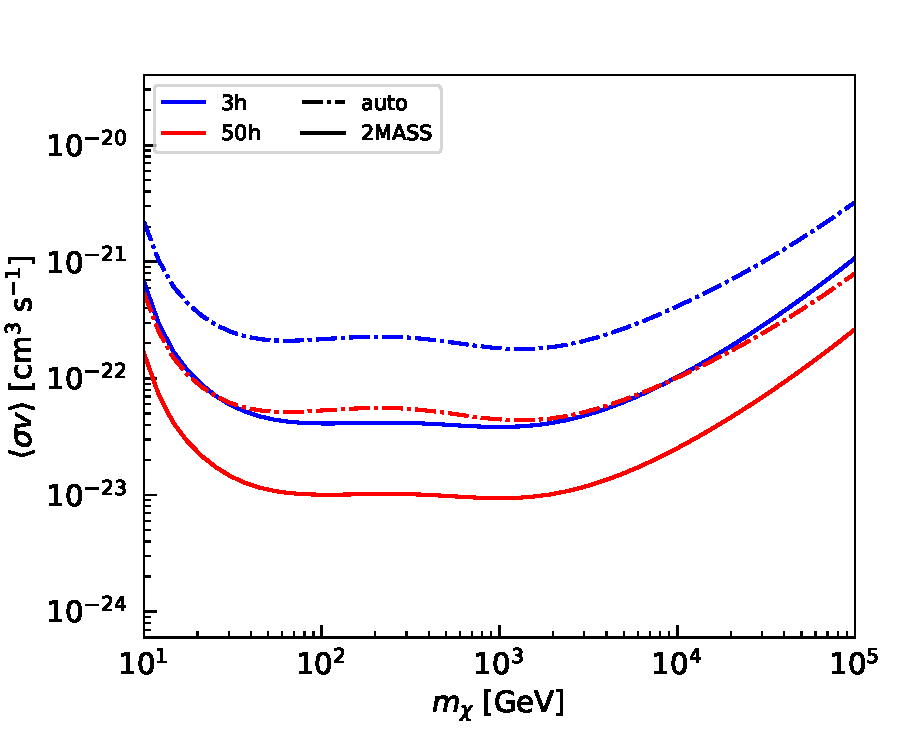
\includegraphics[width=0.45\textwidth]{figures/new_analysis/bounds/sigmav_bound_bb_3-50h.pdf}
    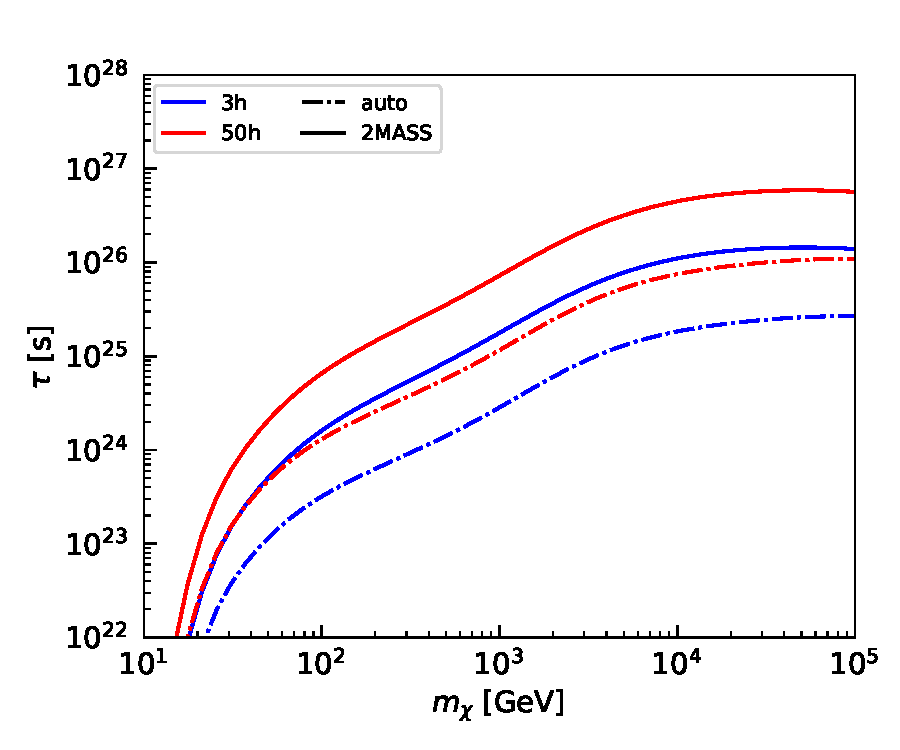
\includegraphics[width=0.45\textwidth]{figures/new_analysis/bounds/tau_bound_bb_3-50h.pdf}
    \caption{Left: Predicted upper bounds on the dark matter cross-section $\langle \sigma v \rangle$, for annihilation into $b\bar{b}$, based on 3-hour and 50-hour of observations. The curves represent the bounds from $\gamma$-ray auto-correlation (dot-dashed) and cross-correlation with the 2MASS galaxy catalog (solid). Right: Same as the left panel, but for the lower bound on the DM particle lifetime $\tau$.}
    \label{fig:bounds1}
\end{figure*}


\begin{figure*}[t!]
    \centering
    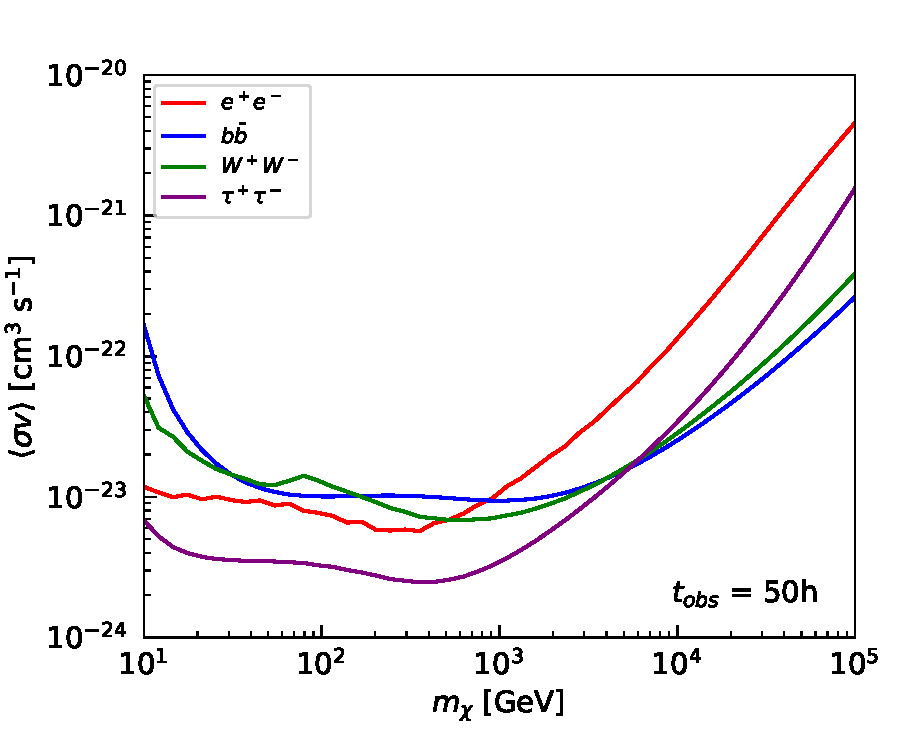
\includegraphics[width=0.45\textwidth]{figures/new_analysis/bounds/sigmav_bound_50h_e_b_W_tau_cross.pdf}
    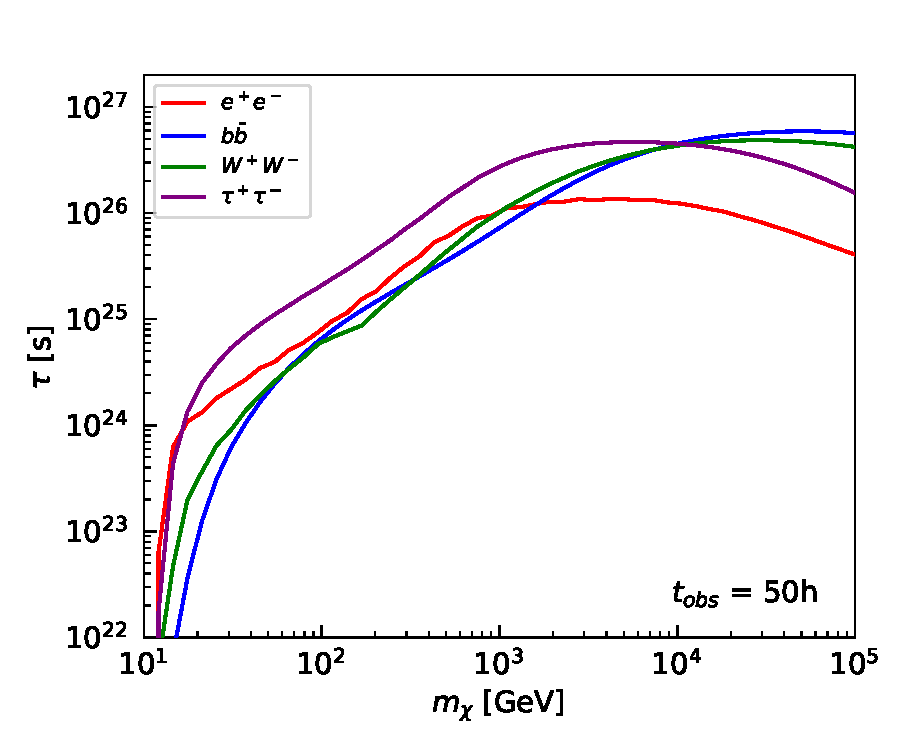
\includegraphics[width=0.45\textwidth]{figures/new_analysis/bounds/tau_bound_50h_e_b_W_tau_cross.pdf}
    \caption{Left: Predicted upper bounds on the dark matter cross-section $\langle \sigma v \rangle$ from the cross-correlation with 2MASS galaxies, based on 50 hours of observation, for various dark matter annihilaton final states: $e^+e^-, b\bar{b}$, $W^+W^-$ and $\tau^+\tau^-$. Right: Same as the left panel, but for the lower bound on the DM particle lifetime $\tau$.}
    \label{fig:all_channels1}
\end{figure*}

\begin{figure*}[t!]
    \centering
    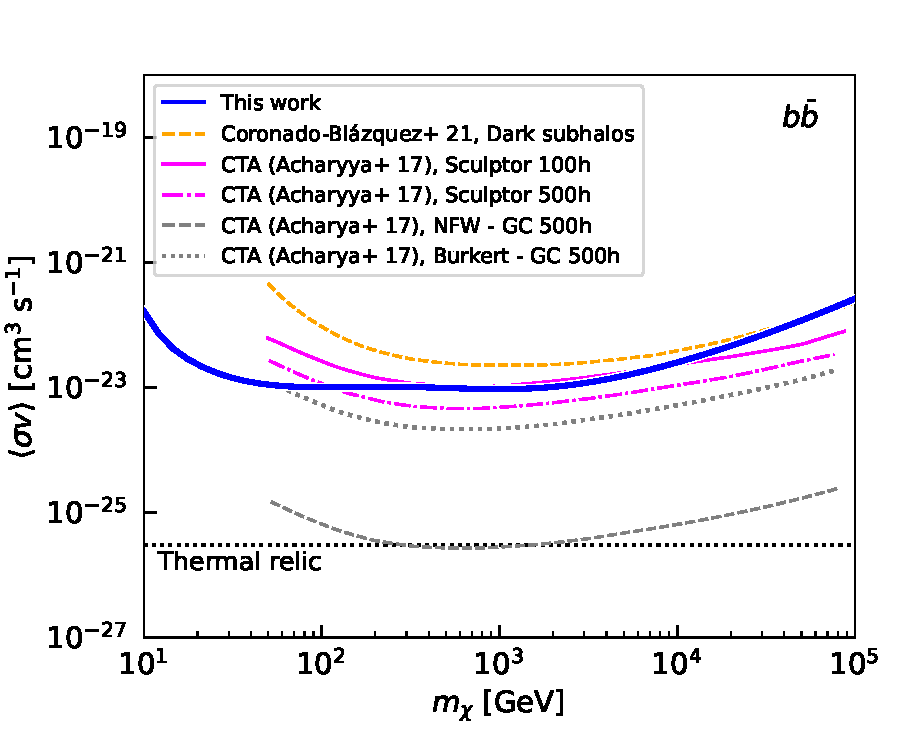
\includegraphics[width=0.45\textwidth]{figures/new_analysis/bounds/sigmav_bound_b_cross+lit-bb-GC.pdf}
    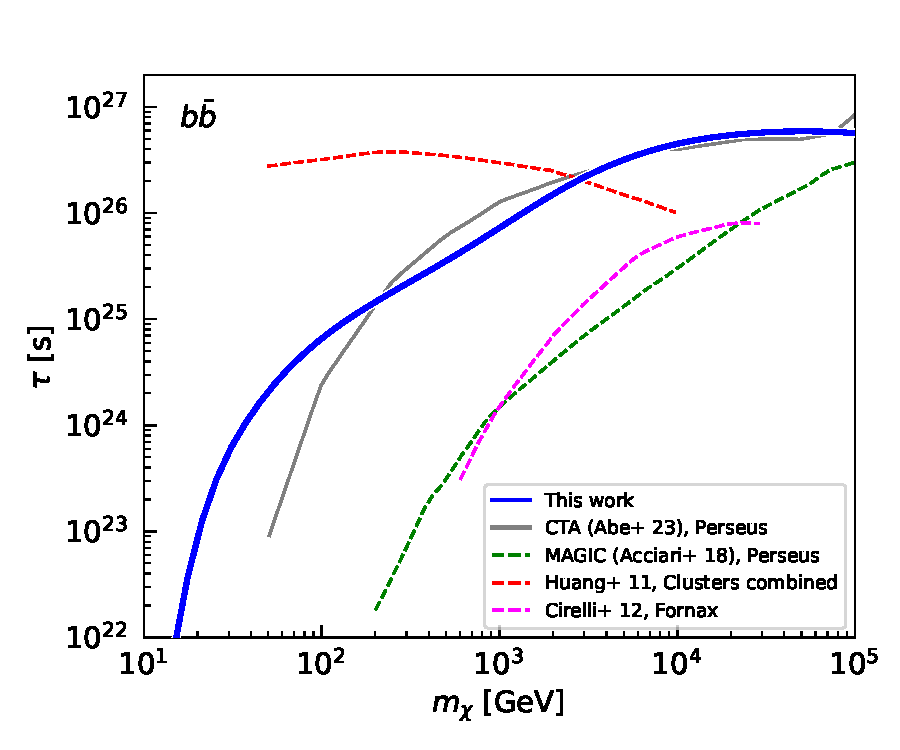
\includegraphics[width=0.45\textwidth]{figures/new_analysis/bounds/tau_bound_50h_b_cross+lit-bb.pdf}
    \caption{Left: Comparison between the forecast on the upper bounds on the annihilation cross-section $\langle\sigma v \rangle$ obtained in this work with other bounds from the literature, for the $b\bar{b}$ annihilation channels: bounds from non-observation of dark sub-halos (dashed yellow) \cite{Coronado_Blazquez_2021}, from Sculptor dwarf galaxy \cite{CTA_2017} with 100 hours (solid magenta) and with 500 hours (dot-dashed magenta) of observations with CTAO. Sensitivities from the Galactic halo have large uncertainties due to the assumptions on the dark matter profile toward the Galactic Center, therefore we show two limiting cases of an NFW profile (dashed gray) and of a cored profile (dotted gray) profiles for 500h with CTAO \cite{CTA_2017}. Right: Comparison between the forecast on the lower bounds on the DM particle lifetime $\tau$ obtained in this work with other bounds from the literature, for the $b\bar{b}$ decay channel: bound from Perseus with CTAO \cite{CTA2023} and MAGIC \cite{MAGIC_2018}, from galaxy clusters \cite{Huang_2012} and from Fornax \cite{Cirelli_2012}.}
    \label{fig:comparison1}
\end{figure*}

\subsection{Dark matter}
We now turn to assessing the CTAO sensitivity to an auto- or cross-correlation APS originating from DM annihilation or decay. To this end, we compare the null hypothesis, where only the contribution from astrophysical sources is present, with the alternative hypothesis scenario in which a DM $\gamma$-ray component is added on top of the astrophysical signal. From this comparison, we derive the minimum DM signal required to be statistically distinguishable from the purely astrophysical case. 

For cross-correlations, we adopt the following test statistics:
\begin{equation}
    \varDelta \chi^2 = \sum_{\ell, i} \left(\frac{C_{\ell, i}^{\gamma_\textrm{astro+DM}g}}{\varDelta C_{\ell, i}^{\gamma_\textrm{astro+DM}g}} \right)^2 - \sum_{\ell, i} \left(\frac{C_{\ell, i}^{\gamma_\textrm{astro}g}}{\varDelta C_{\ell, i}^{\gamma_\textrm{astro}g}} \right)^2\;,
\end{equation}
%
where $\smash{C_{\ell, i}^{ \gamma_\textrm{astro}g}}$ denotes the cross-correlation signal due to the presence of only astrophysical sources, while $\smash{C_{\ell, i}^{ \gamma_\textrm{astro+DM}g}}$ refers to the case where a DM-induced $\gamma$-ray emission is present. The corresponding standard deviations are $\smash{\varDelta C_{\ell, i}^{ \gamma_\textrm{astro}g}}$ and $\smash{\varDelta C_{\ell, i}^{ \gamma_\textrm{astro+DM}g}}$, respectively. Since the DM signal depends on the DM mass $m_\chi$ and scales linearly with the annihilation rate $\langle \sigma v \rangle$ (or inversely with the lifetime $\tau$ in the case of decay), as outlined in {\cref{app:model}}, we derive bounds on the annihilation (or decay) rate by scanning over the DM mass $m_\chi$.
We then derive the $2\,\sigma$ bounds on the annihilation (or decay)
rate by requiring $\varDelta \chi^2 = 4$. A similar test statistic and procedure is employed for the auto-correlation case.
We stress that the DM results are derived assuming the nominal case for the astrophysical sources scenario (i.e., HSP+LISP) and point-source sensitivity.
Nonetheless, the LISP component has no impact on the DM results due to low-energy SED cut-off, as explained in the previous section.
We have also verified that the point-source sensitivity uncertainty discussed in the previous section has a negligible impact on the DM results. To this aim, we explicitly derived DM sensitivities for the two cases of nominal and degraded point-source sensitivity, finding indistinguishable results.




\Cref{fig:bounds1} shows the sensitivity to the DM annihilation and decay in the $b\bar{b}$ annihilation channel, derived from the auto-correlation and cross-correlation APS with the  2MASS catalog, for $3\,\textrm{hrs}$ and $5\,\textrm{hrs}$ of CTAO observations. The $5\,\textrm{hrs}$ case yields approximately a factor of 4 improvement in sensitivity compared to the $3\,\textrm{hrs}$ case, while the cross-correlation outperforms the auto-correlation by approximately a factor of 5. This is expected since in the auto-correlation, the DM signal competes with strong blazar auto-correlation, while in the cross-correlation, the blazar contribution is much lower, yielding a more favorable signal-to-background ratio.
Sensitivities obtained from the cross-correlation with the 2MRS catalog are very similar and are shown {\cref{app:model}}.
Note that in this case, the uncertainty on the point-source detection threshold does not play a significant role, since the DM signal is always diffuse.

\Cref{fig:all_channels1} shows the sensitivities of the cross-correlation technique for different annihilation channels, while \cref{fig:comparison1} provides a comparison with existing results in the literature for alternative DM search strategies. In particular, we show bounds from observations of dwarf galaxies \cite{CTA_2017} and dark sub-halos \cite{Coronado_Blazquez_2021} for DM annihilation, and from galaxy clusters for decaying DM \cite{CTA2023,MAGIC_2018,Huang_2012,Cirelli_2012}. Our results show that the cross-correlation technique is competitive, yielding constraints comparable to those from other methodologies. For comparison, the figure also includes the sensitivity for annihilation in the Galactic halo, for 500 hr of observations with CTAO \cite{CTA_2017}: in this case, the values of $\langle \sigma v \rangle$ that can be probed can be lower, but the reachable bounds are strongly dependent on the assumptions regarding the DM profile near the Galactic Center.

In {\cref{app:modelll}} we show a comprehensive set of plots for different hours of observations and DM channels. 



%%%%%%%%%%%%%%

